\chapter{Background}

\section{Zel'dovich Approximation}
% Taken from the Caustics paper

\label{sec:ZA}

ZA is an elegant analytical approximation to describe the non-linear gravitational evolution of collisionless particles in continuous media. \hl{Technically it is the first order Lagrangian perturbation theory, however Zeldovich suggested to extrapolate it to the beginning of the non-perturbative nonlinear stage and predicted the formation of caustics which are the boundaries of
the first very thin multistream regions dubbed by him  'pancakes'.}
ZA describes a dynamical mapping from the initial Lagrangian coordinates $\mathbf{q}$ to Eulerian positions at time $t$. In comoving coordinates, $\mathbf{x} = \mathbf{r}/a(t)$ (where $\mathbf{r}$ is the physical coordinate  and $a(t)$ is the scale factor; \hl{(?) assuming normalization $a(z=0)=1, \mathbf{r}$ are 
the physical coordinates of particles at present} ), ZA takes the form:

\begin{equation} \label{eq:ZA1}
 \mathbf{x}(\mathbf{q}, D(t) ) = \mathbf{q} + D(t) s(\mathbf{q}) 
\end{equation}

where $D(t)$ is the linear density growth factor, and the the initial density perturbation field $\psi(\mathbf{q})$ determines the potential vector field $\mathbf{s(q)} = - \nabla_q \psi(\mathbf{q})$. 
% The initial cosmic density field is a realization of a Gaussian random process, specified completely by the associated power spectrum, $P(k)$. 
Mass conservation formalism implies $\rho(\mathbf{x}, t) d\mathbf{x} = \rho_0 d\mathbf{q} $, so the density field at $t>0$ in terms of Lagrangian coordinates is given as 

\begin{equation}
 \rho(\mathbf{q}, t) = \rho_0 J \left[ \frac{\partial\mathbf{x}}{\partial\mathbf{q}} \right]^{-1}
\end{equation}

where the Jacobian $J \left[ \frac{\partial\mathbf{x}}{\partial\mathbf{q}} \right]$ is calculated using Equation \ref{eq:ZA1}. Moreover, diagonalization of the resulting real, symmetric deformation tensor $d_{ij} = - \nabla_q \mathbf{s(q)} =  \partial^2 \psi(\mathbf{q})/ \partial q_i \partial q_j$ in terms of its eigenvalues $\lambda_1(\mathbf{q})$, $\lambda_2(\mathbf{q})$, $\lambda_3(\mathbf{q})$ gives the contraction or expansion along the three principal axes. This reduces the mass density to a convenient form:

\begin{equation}
 \rho(\mathbf{q}, t) = \frac{\rho_0}{ \left[1 - D(t) \lambda_1(\mathbf{q}) \right]\left[1 - D(t) \lambda_2(\mathbf{q}) \right]\left[1 - D(t) \lambda_3(\mathbf{q}) \right] }
\end{equation}

Since the deformation tensor $d_{ij}$ and its eigenvalues depend only on the initial density field, the ordered eigenvalues defined in Lagrangian space $\lambda_1(\mathbf{q}) \geq \lambda_2(\mathbf{q}) \geq \lambda_3(\mathbf{q})$ determine collapse condition for masses in Eulerian space (see \cite{Doroshkevich1973} and \cite{Lee1998} {for the PDFs  of the eigen values as well as several other parameters} in the case of Gaussian random fields). In the context of this paper, formation of caustics is of much interest: with increasing $D(t)$, the mass density rises until reaching singularity at $D(t) = 1/\lambda_3(\mathbf{q})$. In \hl{Lagrangian space, the caustics stem from these points and their counterparts  in Eulerian space} were proposed by Zel'dovich as the \hl{'birthplaces' of the first} collapsed structure by gravitational clustering. Now \hl{the regions bounded by the caustic surfaces} are referred to as {\it Zel'dovich pancakes}. The collapse along other principal axes correspond to formation of filaments and knots (\cite{Arnold1982}, \hl{Shandarin and Klypin (1984), however simultaneous collapses along all three eigen axes never happen in the case of generic flows.})

\begin{figure} 
\centering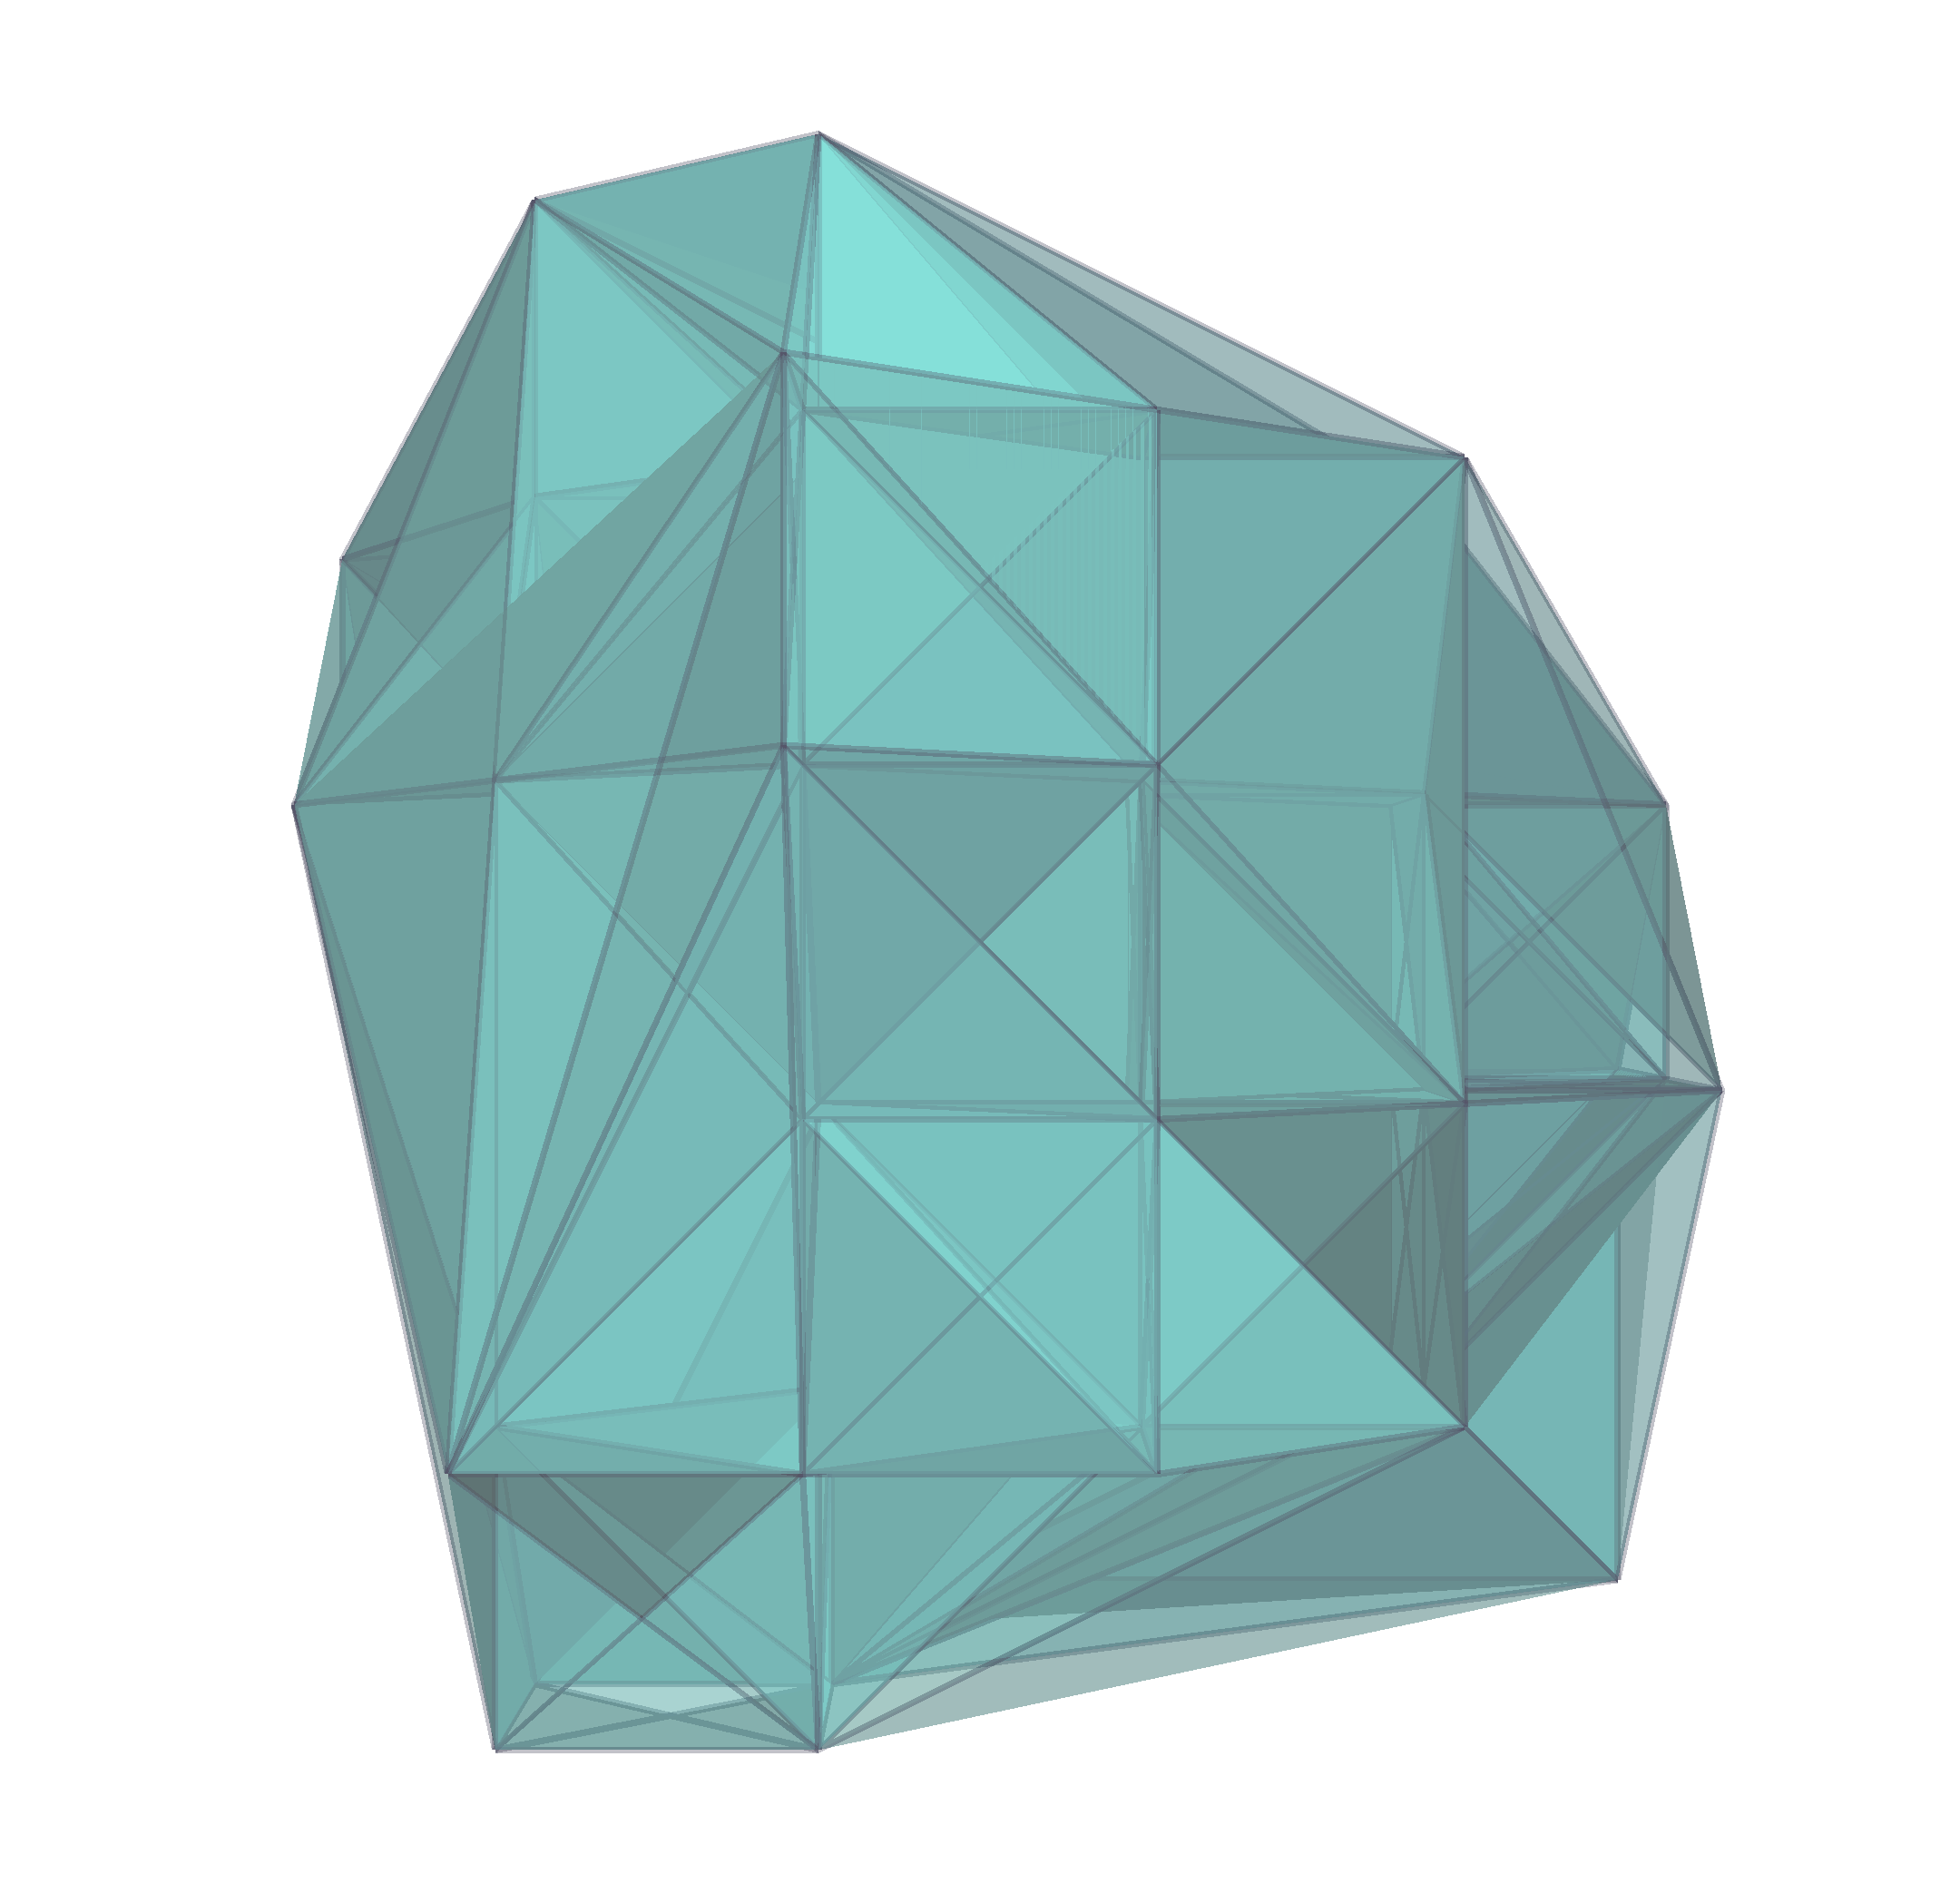
\includegraphics[width=9cm]{Chapter2/Plots/qDel.png}
\centering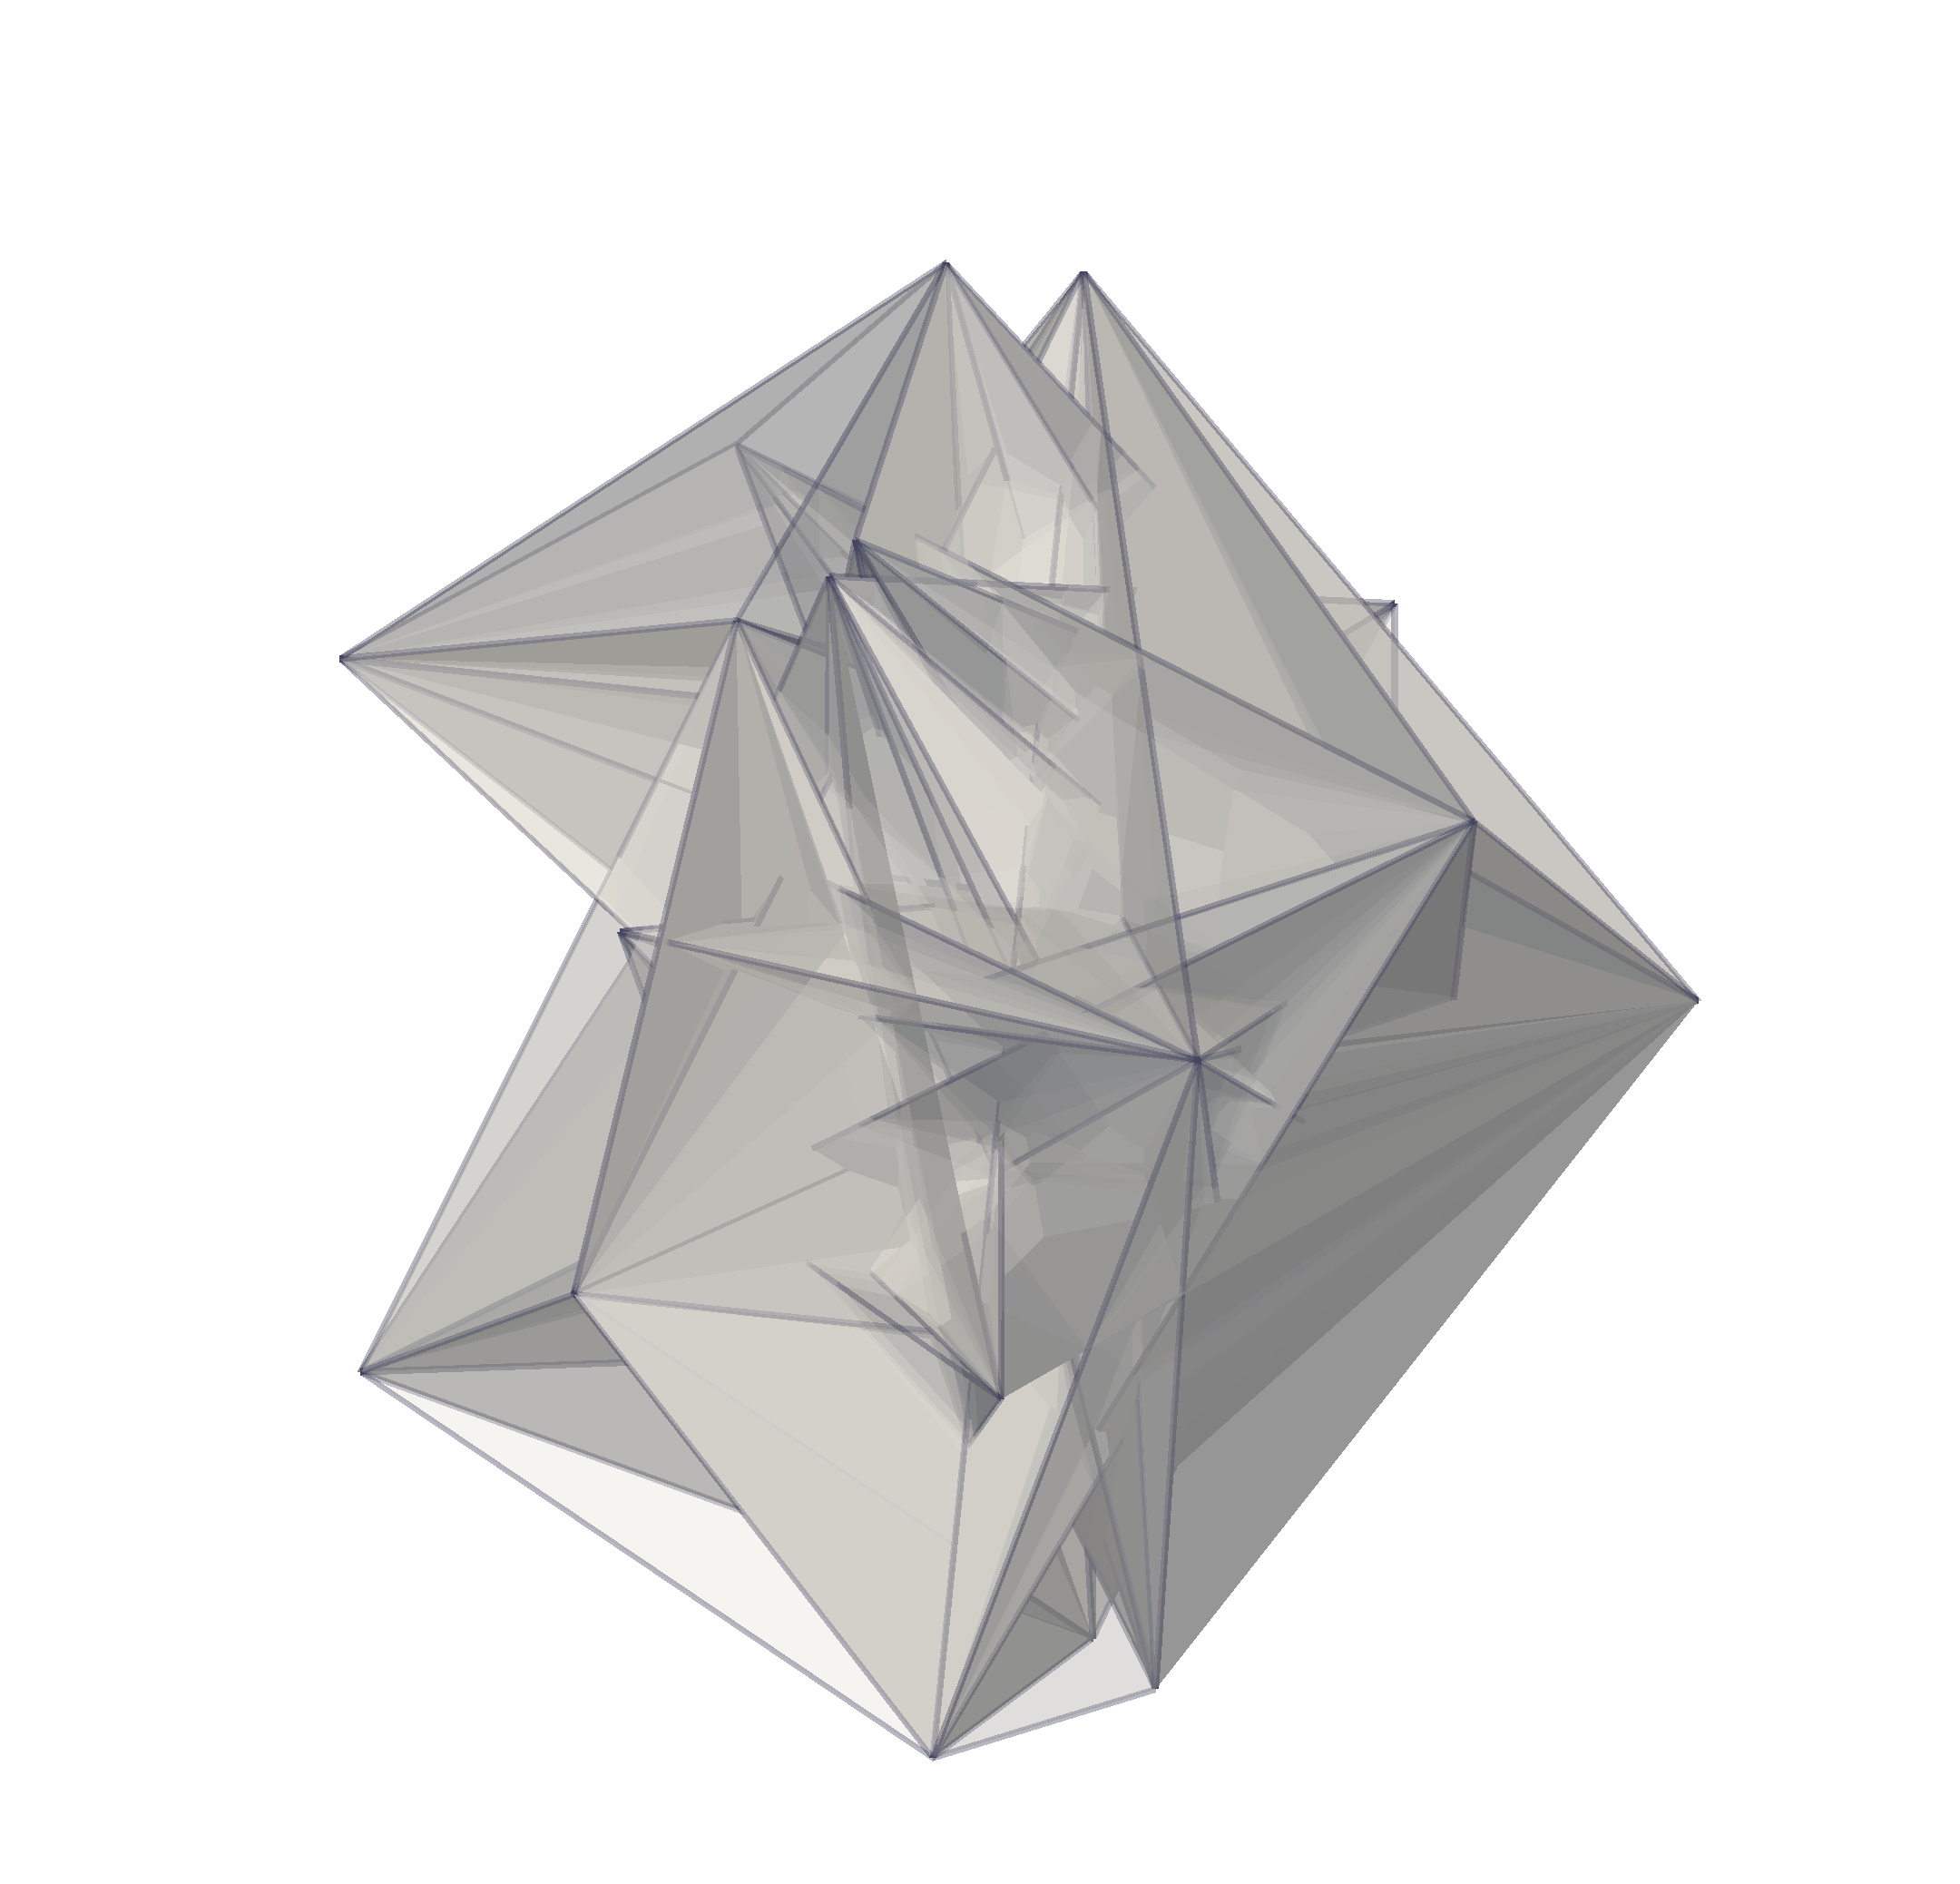
\includegraphics[width=5cm]{Chapter2/Plots/x.png}
\caption{ This plot shows the idea of Lagrangian tessellations. Left: The distribution of Dark matter particles in Lagrangian space is on the regular grid. The tetrahedra surfaces in this case are mostly regular (except at the edges). Right panel shows the Eulerian positions of the same particles at $z=0$. The particles clearly have undergone multiple flip-flops, and the intersections of Lagrangian tetrahedra signifies locations of caustic surfaces. Specific tessellation schemes can be utilized separately to identify these surfaces. }
\label{fig:Tess}
\end{figure}


Furthermore, the analytical understanding of these structures are thoroughly complicated: In a 2-dimensional ZA, for example, there are 
\hl{only two types of fundamental singularities that exist at generic instants of time($A_2$, which are lines and $A_3$, which are the cusp points of $A_2$ lines).   In addition there are two singular points ($A_4$, and $D_4$) that exist  only at particular instants of time: at $A_4$ two cusp $A_3$-points are formed and a smooth part of an $A_2$ line is  transformed in self-crossing
line. Moreover there are  
 In addition there are several transient forms that exist only 
at particular times.}
Each of these correspond of formation, mergers, branching and other dynamical processes involving pancakes. \cite{Arnold1982} and \cite{Hidding2014} studied of singularities in 2-dimensional collapse) in exhaustive detail, but similar analytical characterization of 3-dimensional ZA has not been satisfactorily done yet.  
 
 
Complexities in 3-dimensional caustics is partly due the intricate mapping in the hypersurface $\mathbf{x}(\mathbf{q})$ called the Lagrangian submanifold (See Figure \ref{fig:Tess}). 
\hl{The Lagrangian submanifold $\mathbf{x}(\mathbf{q})$  is a single valued, smooth and differentiable function in it's 6-dimensional space $(\mathbf{q}, \mathbf{x})$, however the projection onto 3-dimensional Eulerian space is entangled with creases, kinks and folds (Note that this  submanifold is very different than the phase space $(\mathbf{x},\mathbf{v})$, even though they are connected by a cannonical transformation).} However, dilineating the Lagrangian submanifold reveals several properties of the dark matter dynamics not inferred from position-space analyses. Two fields related to tessellating the Lagrangian submanifold -- The Multistream field $n_{str}(\mathbf{x})$ in Eulerian space and the Flip-Flop field $n_{ff}(\mathbf{q})$ in Lagrangian space (check \cite{Shandarin2012}, \cite{Ramachandra2015}, \cite{Shandarin2016}) are closely related. 


\section{The multistream flow field in one-dimension}
% Taken from appendix A
\label{appendix:nstream}

\begin{figure}
\begin{minipage}[t]{.99\linewidth}
  \centering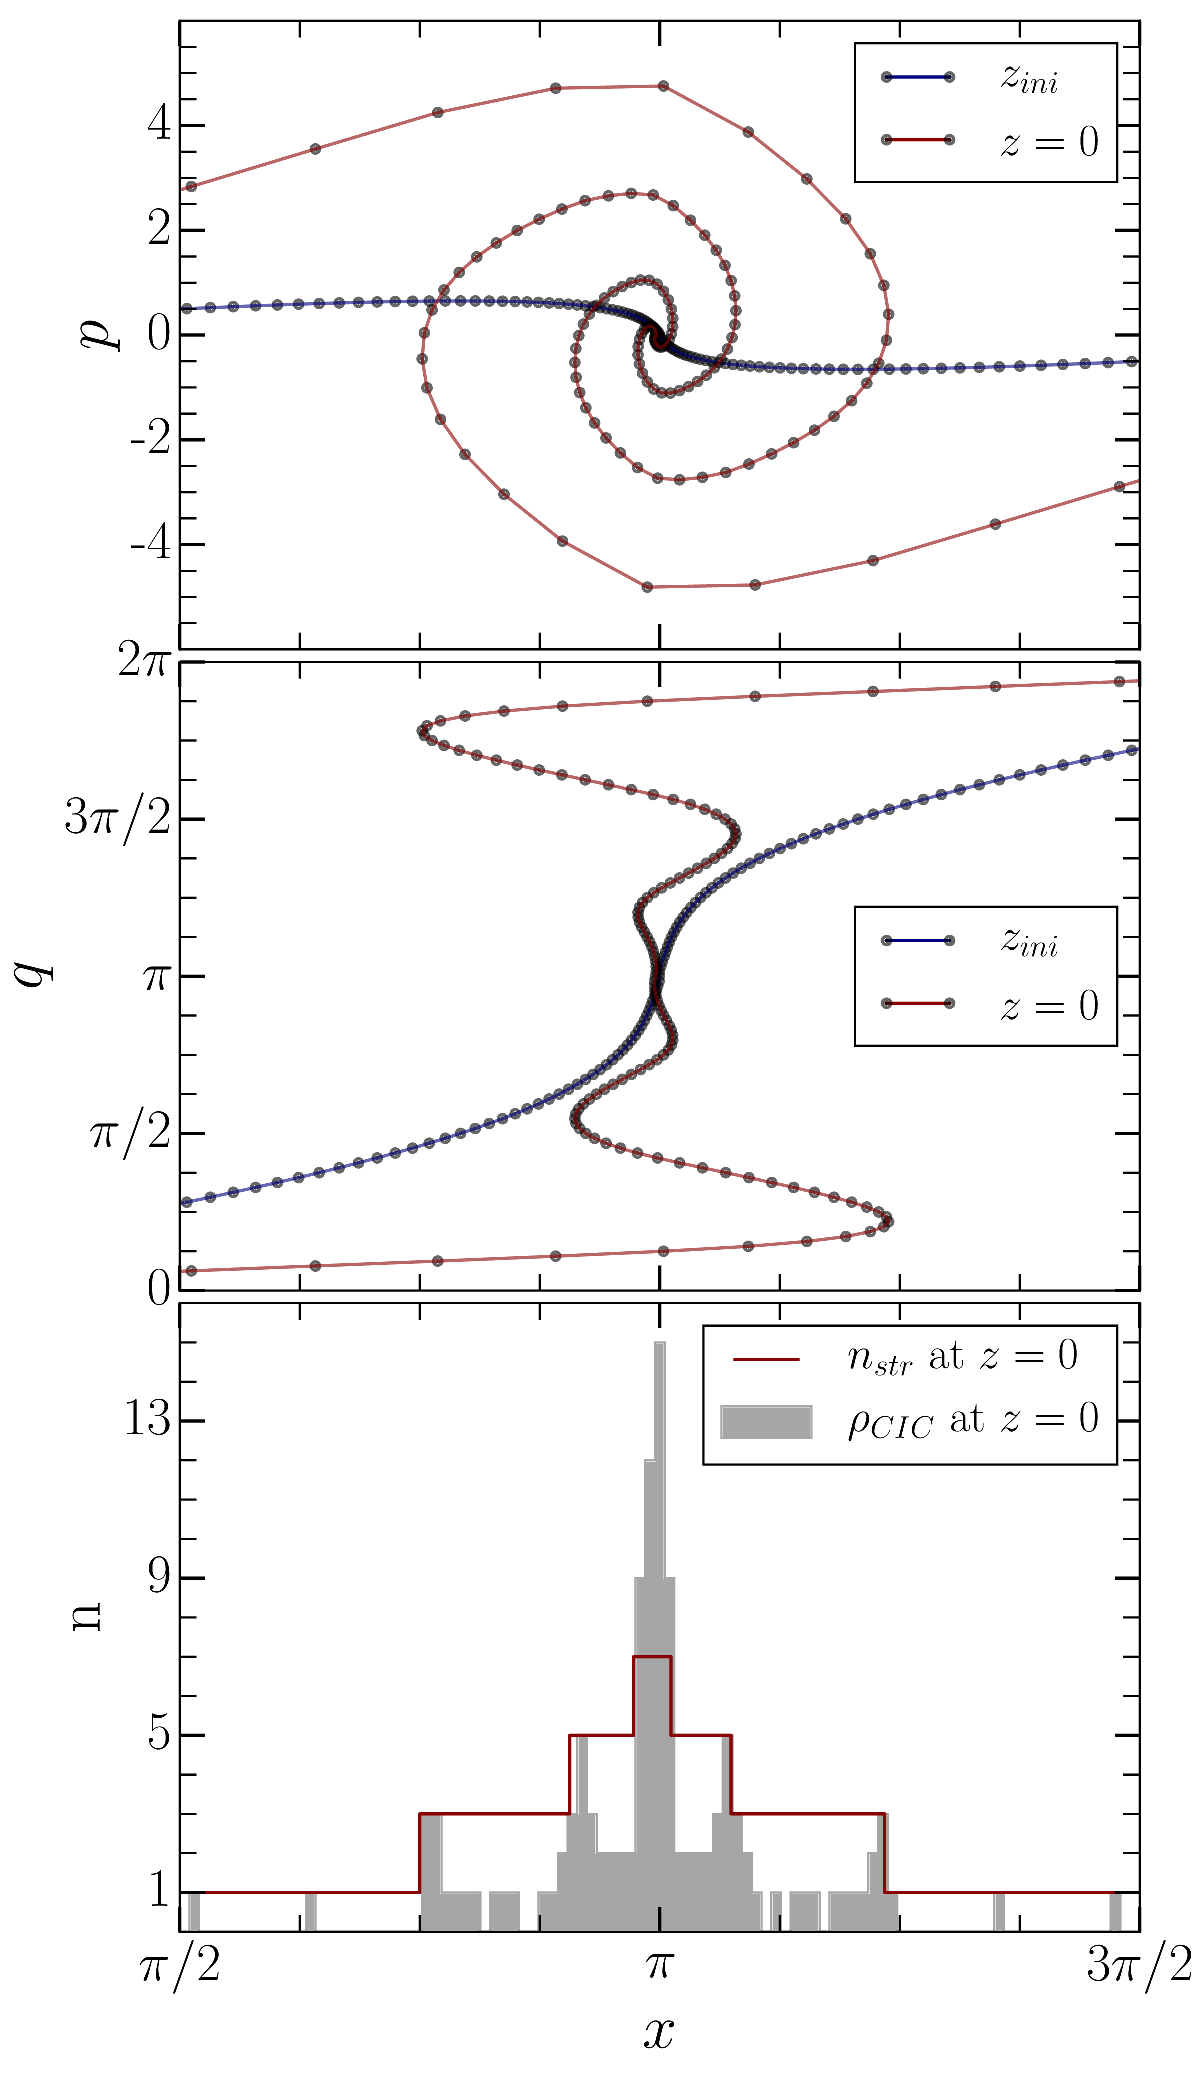
\includegraphics[width=8.cm]{Chapter4/Source_v2/fig13.pdf} 
\end{minipage}\hfill
\caption{ Multi-streaming in one-dimension gravitational collapse. Top panel: $(\bf{p}, \bf{x})$ phase-space representation redshift $z_{ini}$ and $z = 0$. Dots represent the dark matter particles. Initially the mass particles are in the linear stage of evolution. At $z = 0$, multiple values of $\bf{p}(\bf{x})$ is seen in the collapsed regions. Middle panel: Equivalent Lagrangian sub-manifold $\bf{q}(\bf{x})$. At $z_{ini}$, the dashed line represents $\bf{q} = \bf{x}$. Number of streams are parametrized from this sub-manifold. Bottom panel: The multistream field $n_{str}$ and the number-density using CIC algorithm, $n_{CIC}$ at $z = 0$. }
\label{fig:phase1d}
\end{figure}

The top panel in \autoref{fig:phase1d} shows the velocity multistreaming phenomenon in a one-dimensional collapse. The phase-space $(\bf{p}, \bf{x})$ (where $p$ is the momentum and $x$ is the co-moving Eulerian coordinate) is single-valued in the linear stage of evolution (at redshift $z_{ini}$). Non-linear stage of gravitational evolution of the collision-less dark matter particles then results in multi-valued $\bf{p} (\bf{x},z)$ at $z = 0$. The mass particles are sparsely  distributed outside the region of gravitational collapse, and are denser in the inner streams.

 
A dynamically equivalent transformation $(\bf{p}, \bf{x}) \mapsto (\bf{q}, \bf{x}) $ (where $\bf{q}$ is the Lagrangian coordinate) shows the Lagrangian sub-manifold in the middle panel of \autoref{fig:phase1d}. This two-dimensional phase-space has foldings that correspond to multiple velocity streams, although the sub-manifold itself remains continuous. A projection of the Lagrangian sub-manifold at each point in the configuration space quantifies the number-of-streams. Folding in the sub-manifold are checked for points in configuration space using tessellations. The tessellating simplices in one-dimensional model are just the line-segments whose nodes are the dark matter particles in the Lagrangian space. Dynamical property is accounted for in this phase-space tessellation since labels of the nodes remain intact throughout the evolution; the line segments may shorten, extend or change orientation. Each folding in the Lagrangian sub-manifold increases the number of streams by a factor of two. In three-dimensional simulations, the sub-manifold twists in complicated ways in a six-dimensional phase space. The number-of-streams in N-body simulations (\citealt{Shandarin2012} and \citealt{Abel2012}) is calculated using Lagrangian/phase-space tessellations. This triangulation is conceptually different from the Voronoi (See \citealt{Schaap2000} and references therein) or Delaunay \citep{Icke1991} tessellation schemes. 

The bottom panel \autoref{fig:phase1d} shows the the multistream field $n_{str}(\bf{x})$ at $z = 0$. The field only takes the values of 1, 3, 5 and 7 in this scenario. Caustics occur at the folds in Lagrangian sub-manifold, and have a measure zero (study of caustics in one- and  two-dimensional evolution is done in \cite{Hidding2014}, three-dimensional caustic surface in a cosmological simulation is shown in \autoref{fig:NstrCaust}). Several properties of the multistream field are significantly different from mass density. The bottom panel also shows an illustration of CIC algorithm (cf. \citealt{Hockney1988}) in calculating density, which is numerically equivalent to counting the number of particles on each cell of a regular grid. One major difference is in the regions before gravitational collapse: $n_{str}$ is universally equal to unity, whereas number density fluctuates. It should also be noted that density by definition is a continuous field; numerical approximations like CIC discretise the field. Alternatively, multistream field is intrinsically a discrete-data field.  



\section{Dynamics: Lagrangian sub-manifold}
Multi-stream flows, Caustics, Flip-flips